Затухание градиентов --- одна из проблем GAN-ов. Предположим, что мы имеем ситуацию, похожую на изображенную на рисунке \ref{fig:7_problem}. В таком случае, как видно, дискриминатор может провести линию так, чтобы идеально (или в целом почти идеально, сути дела не меняет) разделить два класса. Это здорово, но не очень.

Если классы идеально разделились дискриминатором, то $D(x_i) = 1$ для любого $x_i$ в $X$, т.е. для всех объектов первого класса он вернул 1. Для всех же сгенерированных объектов $D(\hat{x_j}) = D(G(z_j)) = 0$ для любого $z_j$~в~$Z$.

Вспомним, как выглядит функция потерь:

\begin{equation}
	L(D, G) = - \frac{1}{n} \sum\limits_{x_i\in X}\log D(x_i) - \frac{1}{n} \sum\limits_{z_j\in Z}\log [1 - D(G(z_j))]
	\label{eq:7_loss}
\end{equation}

Подставим получившиеся значения в функцию потерь \ref{eq:7_loss}:

\begin{equation}
	L(D, G) = - \frac{1}{n} \sum\limits_{x_i\in X}\log 1 - \frac{1}{n} \sum\limits_{z_j\in Z}\log [1 - 0] = 0 = \text{const}
\end{equation}

Константа в том смысле, что нет зависимости от весов генератора или дискриминатора. Это значит, что градиент функции потерь оказывается равным нулю, т.е. ни дискриминатор, ни генератор более не обучаются, поскольку веса не обновляются. Ну понятно, что картинка эта далека от того, чего мы на самом деле хотим, так что это проблема.

\begin{figure}[H]
	\centering
	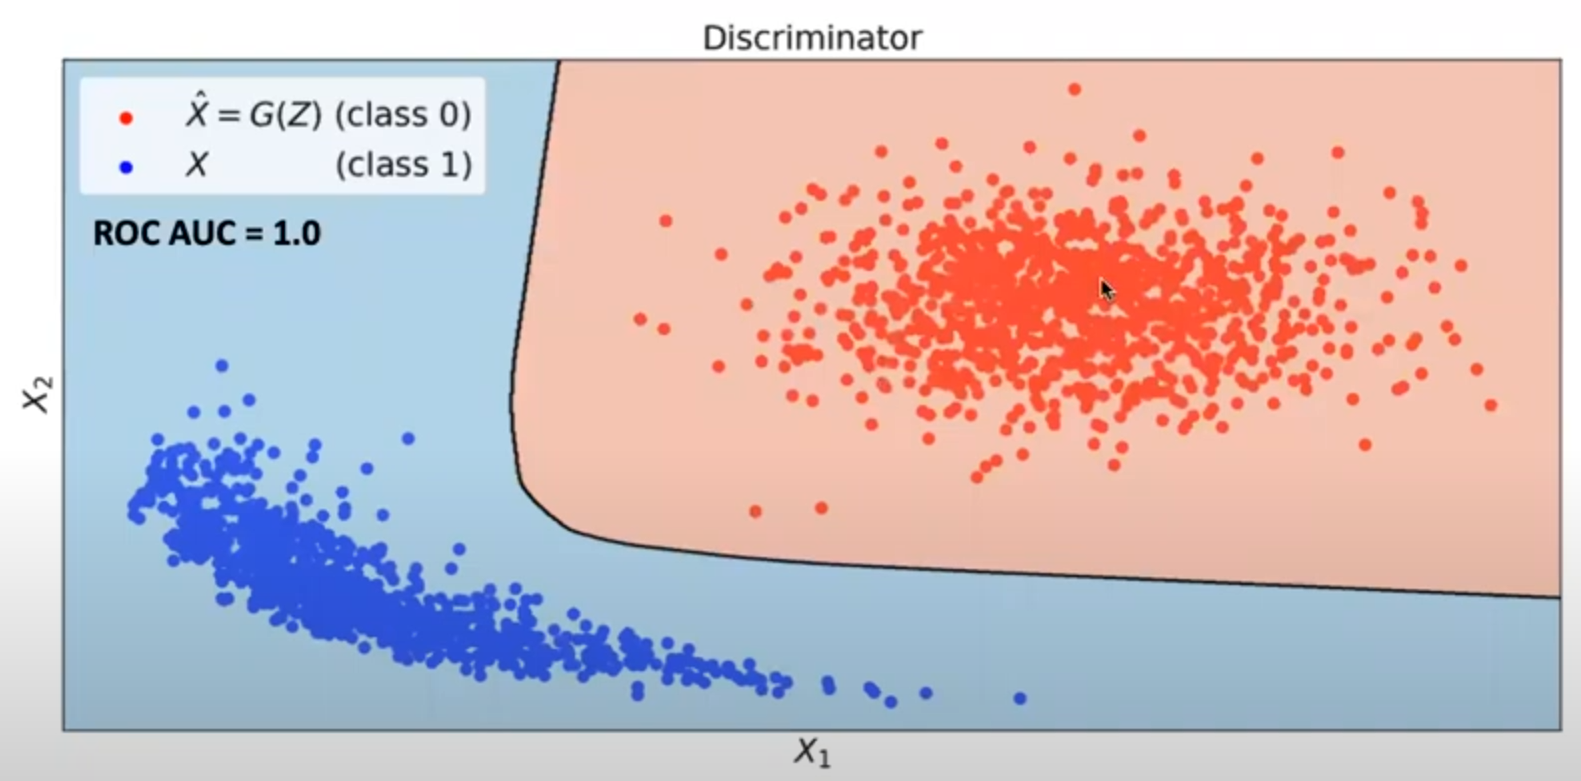
\includegraphics[width=\linewidth]{7_problem}
	\caption{Ситуация, возникшая на некоторой итерации обучения GAN и ведущая к затуханию градиентов}
	\label{fig:7_problem}
\end{figure}